\chapter{Implementation}
In this chapter the implementation steps are introduced of the system described in 
\ref{chap:system_design}. Two LIDAR sensors are placed on a simulated quadcopter in Gazebo, 
that cover the top and bottom hemispheres around the drone. Using the data collected in the
simulator, these range measurements are filtered to simulate a number of VL53L1X sensors with 
a predefined operating modes and orientations. 

In order to simulate the VL53L1X sensors accurately a set of parameters, capabilities and 
limitations of the LIDAR sensor is measured. Data is collected using selected operating modes
on selected distances that are described in \ref{sect:vl53l1x_measurements}. Average distance,
standard deviation, sampling rate and typical range status are extracted. 

The two main components in the evaluation of VL53L1X sensor are a microcontroller and a PC. The 
microcontroller communicates with the sensor and sends the raw measurements to the PC that runs 
data processing and evaluates the received data. I chose to separate data collection and processing,
because data processing is significantly easier in high level programming languages, like Python and 
is much easier to adjust.It also enables data collection and offline processing.


\section{VL53L1X measurement setup}
For each measurement a combination of parameters need to be configured on VL53L1X, these are the 
timing budget, resolution and distance preset. The configuration is done via I2C protocol by the
microcontroller. VL53L1 API from STMicroelectronics is used for interfacing the sensor with the most
recent version at the time: 2.3.3. After completing boot the recommended initialization steps are 
used, as described in example codes and the API user manual \cite{VL53L1XAPIManual}.

Each measurement is triggered in single shot mode, that means exactly one ranging is done by the 
sensor and afterwards it waits until a new command arrives.  Single shot is preferred over continuous
measurements, because if the resolution is set to higher than 1x1, measurements need to be done on 
multiple ROIs and ROI has to be configured before triggering each measurement. In continuous mode 
the ROI cannot be modified between measurements.
A scan is complete if ranges are done on all ROIs of interest. The completed scan is then forwarded 
for processing to the PC via USB-CDC protocol.

\begin{figure}[ht]
    \centering
    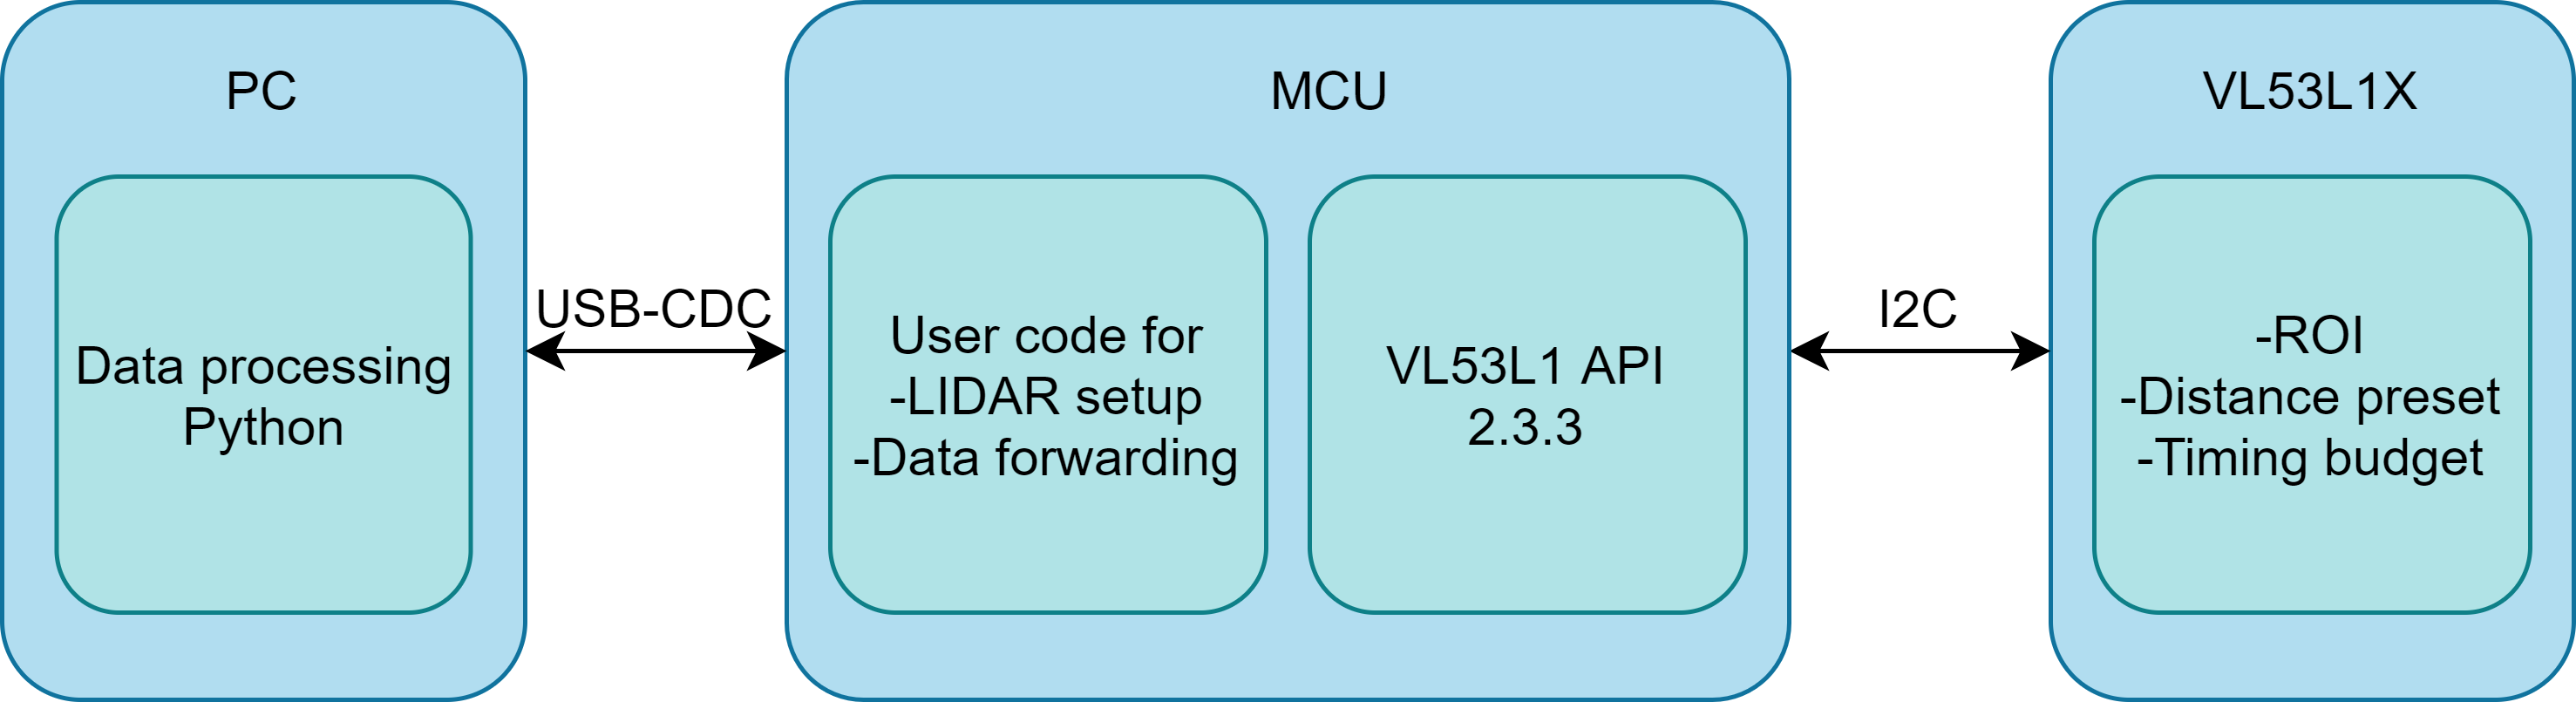
\includegraphics[width=130mm, keepaspectratio]{figures/vl53l1x_workflow.png}
    \caption{VL53L1X measurement workflow}
    \label{fig:vl53l1x_workflow}
\end{figure}


I chose Python as a programming language to read data from USB-CDC protocol and process the incoming
data, because Python is rich in data processing tools and enables quick development. The script first
reads 50 scans coming from the MCU, then closes communication and works on the collected data. 
The features extracted area the average distance, standard deviation, typical range status and sampling
time. Average and standard deviation are calculated based on the whole population as in equations 
\ref{eq:avg} and \ref{eq:std}, where s and r are the indices of scan and range, S and R are the 
number of scans and ranges accordingly.

\begin{equation} \label{eq:avg}
    d_{avg}=\frac{1}{S \cdot R}\sum_{s=0}^S{\sum_{r=0}^R{d_{sr}} } 
\end{equation}

\begin{equation} \label{eq:std}
    d_{std}=\sqrt{ \frac{1}{S\cdot R}\sum_{s=0}^S{ \sum_{r=0}^R{ (d_{sr} -d_{avg}})^2 }}
\end{equation}


\subsection{Comparison of selected operating modes}
VL53L1X LIDAR sensor has an adjustable timing budget from 18.5ms all the way to 1 second, that 
determines the maximum time a ranging operation can take. To see the effect of timing budget with 
different ROI setups and distance modes, 4 timing budgets have been selected. 

With 18.5ms budget the sensor operates on the highest possible measurement frequency of 50Hz. This
can only be achieved in short distance mode without the possibility of modifying the ROI. The second
selected budget is 33ms, that is the lowest possible value to be used with long distance preset.
140ms is the lowest value that can provide measurements up to 4 meters. Lastly 200ms budget is 
selected to see how a higher timing budget affects accuracy. It is also the value used in the 
VL53L1X datasheet\cite{VL53L1XDatasheet} to demonstrate ranging accuracy.

The calculated average distance and standard deviation against the real distance can be seen on 
figure \ref{fig:vl53l1x_meas_opmodes}, std separatle is on \ref{fig:vl53l1x_meas_opmodes_std}. 
The measured sampling time accordingly is visible on figure \ref{fig:vl53l1x_meas_opmodes_sampling}. 

Based on the completed measurements, it can be seen that sampling time is independent from the
distance preset in use and is directly proportional to the number of ROIs in a scan and the 
timing budget. 50Hz sampling rate is not achieved even with 18.5ms timing budget, because 
the LIDAR was used in single shot mode and each measurement needs to be triggered by the MCU.
Sampling time can be increased for setups with 1x1 resolutions by switching to continuous 
measurement mode.

In every setup on each distance the most accurate measurement is always with
resolution 1x1. By increasing the resolution, therefore lowering the receiver SPAD array size,
the measured distance starts to deviate from the real distance and STD increases.This can be
seen on 2.5m distance with medium preset. Long distance preset however produces more accurate 
measurements even on 3m, so it is preferred over medium preset.

Measurements with long distance preset and 140ms timing budget follows the real distances
even on 3 meters, but starts to deviate on 3.5 meters with 2x2 resolution and above. Raising
the timing budget to 200ms reduces the error and standard deviation, but doesn't eliminate 
completely.


\begin{figure}[ht]
    \centering
    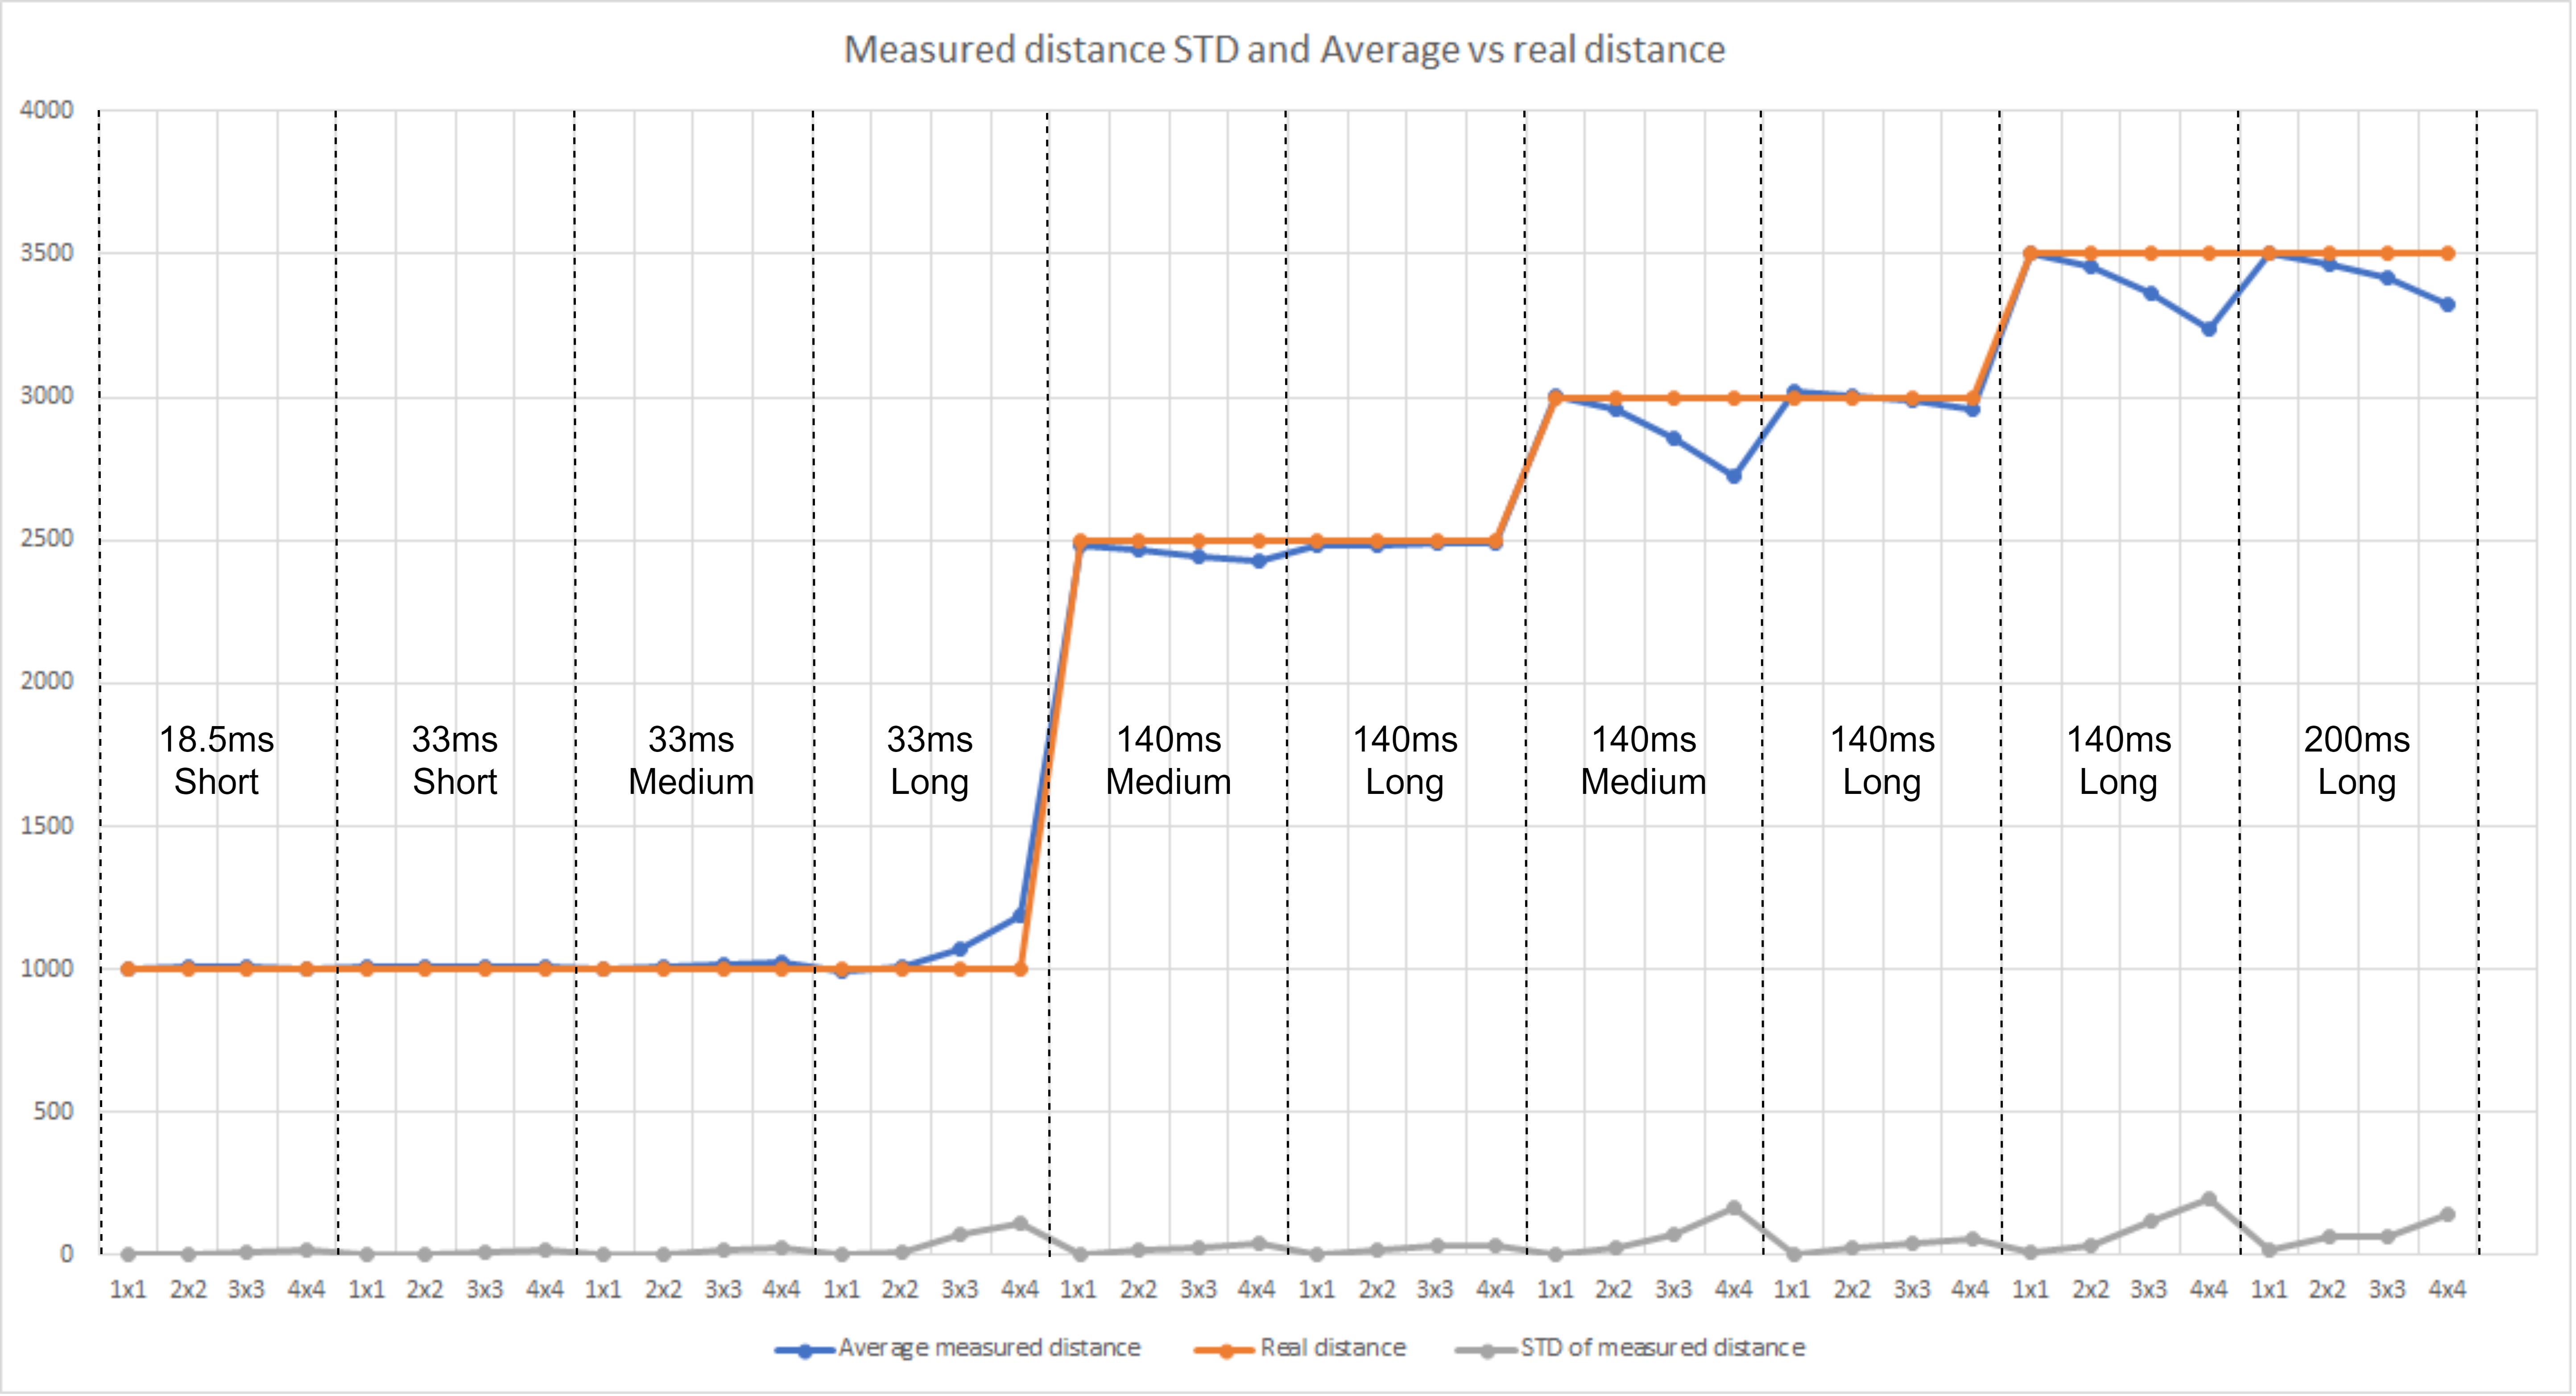
\includegraphics[width=150mm, keepaspectratio]{figures/vl53l1x_measurements_opmodes.png}
    \caption{VL53L1X measured distance STD and Average against real distance}
    \label{fig:vl53l1x_meas_opmodes}
\end{figure}
\begin{figure}[!h]
    \centering
    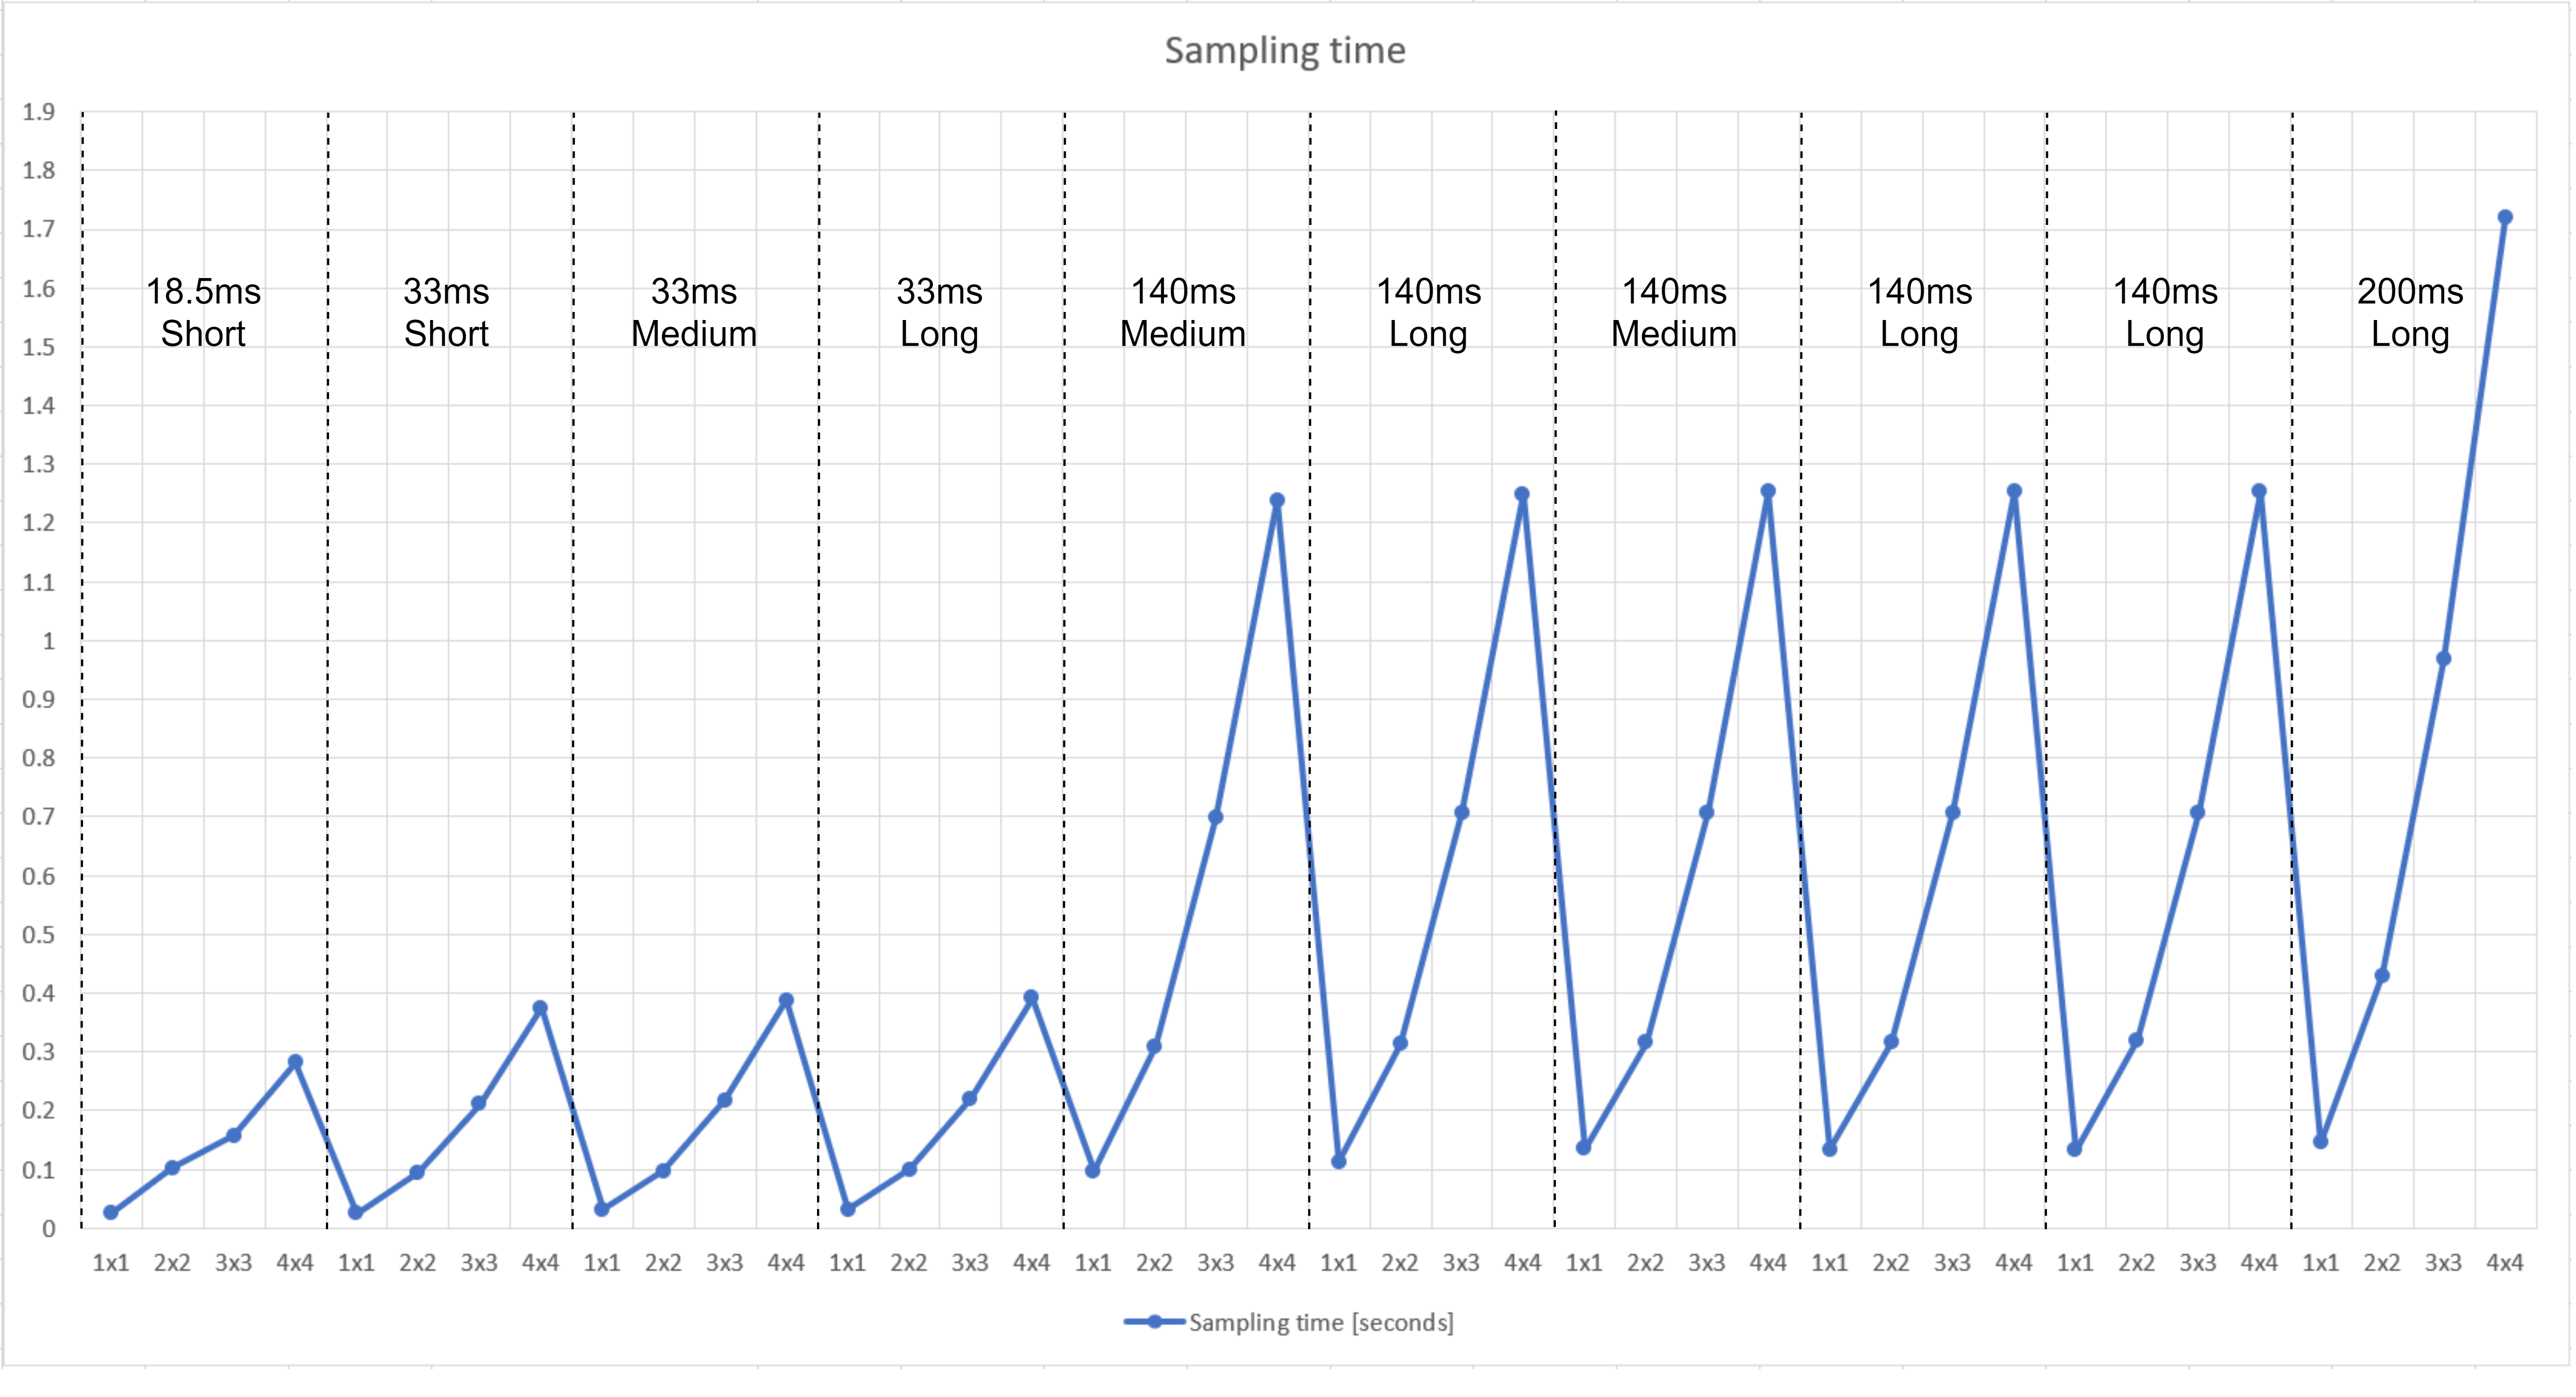
\includegraphics[width=150mm, keepaspectratio]{figures/vl53l1x_measurements_opmodes_sampling.png}
    \caption{VL53L1X range sampling time in different operation modes}
    \label{fig:vl53l1x_meas_opmodes_sampling}
\end{figure}

\newpage

\begin{figure}[!h]
    \centering
    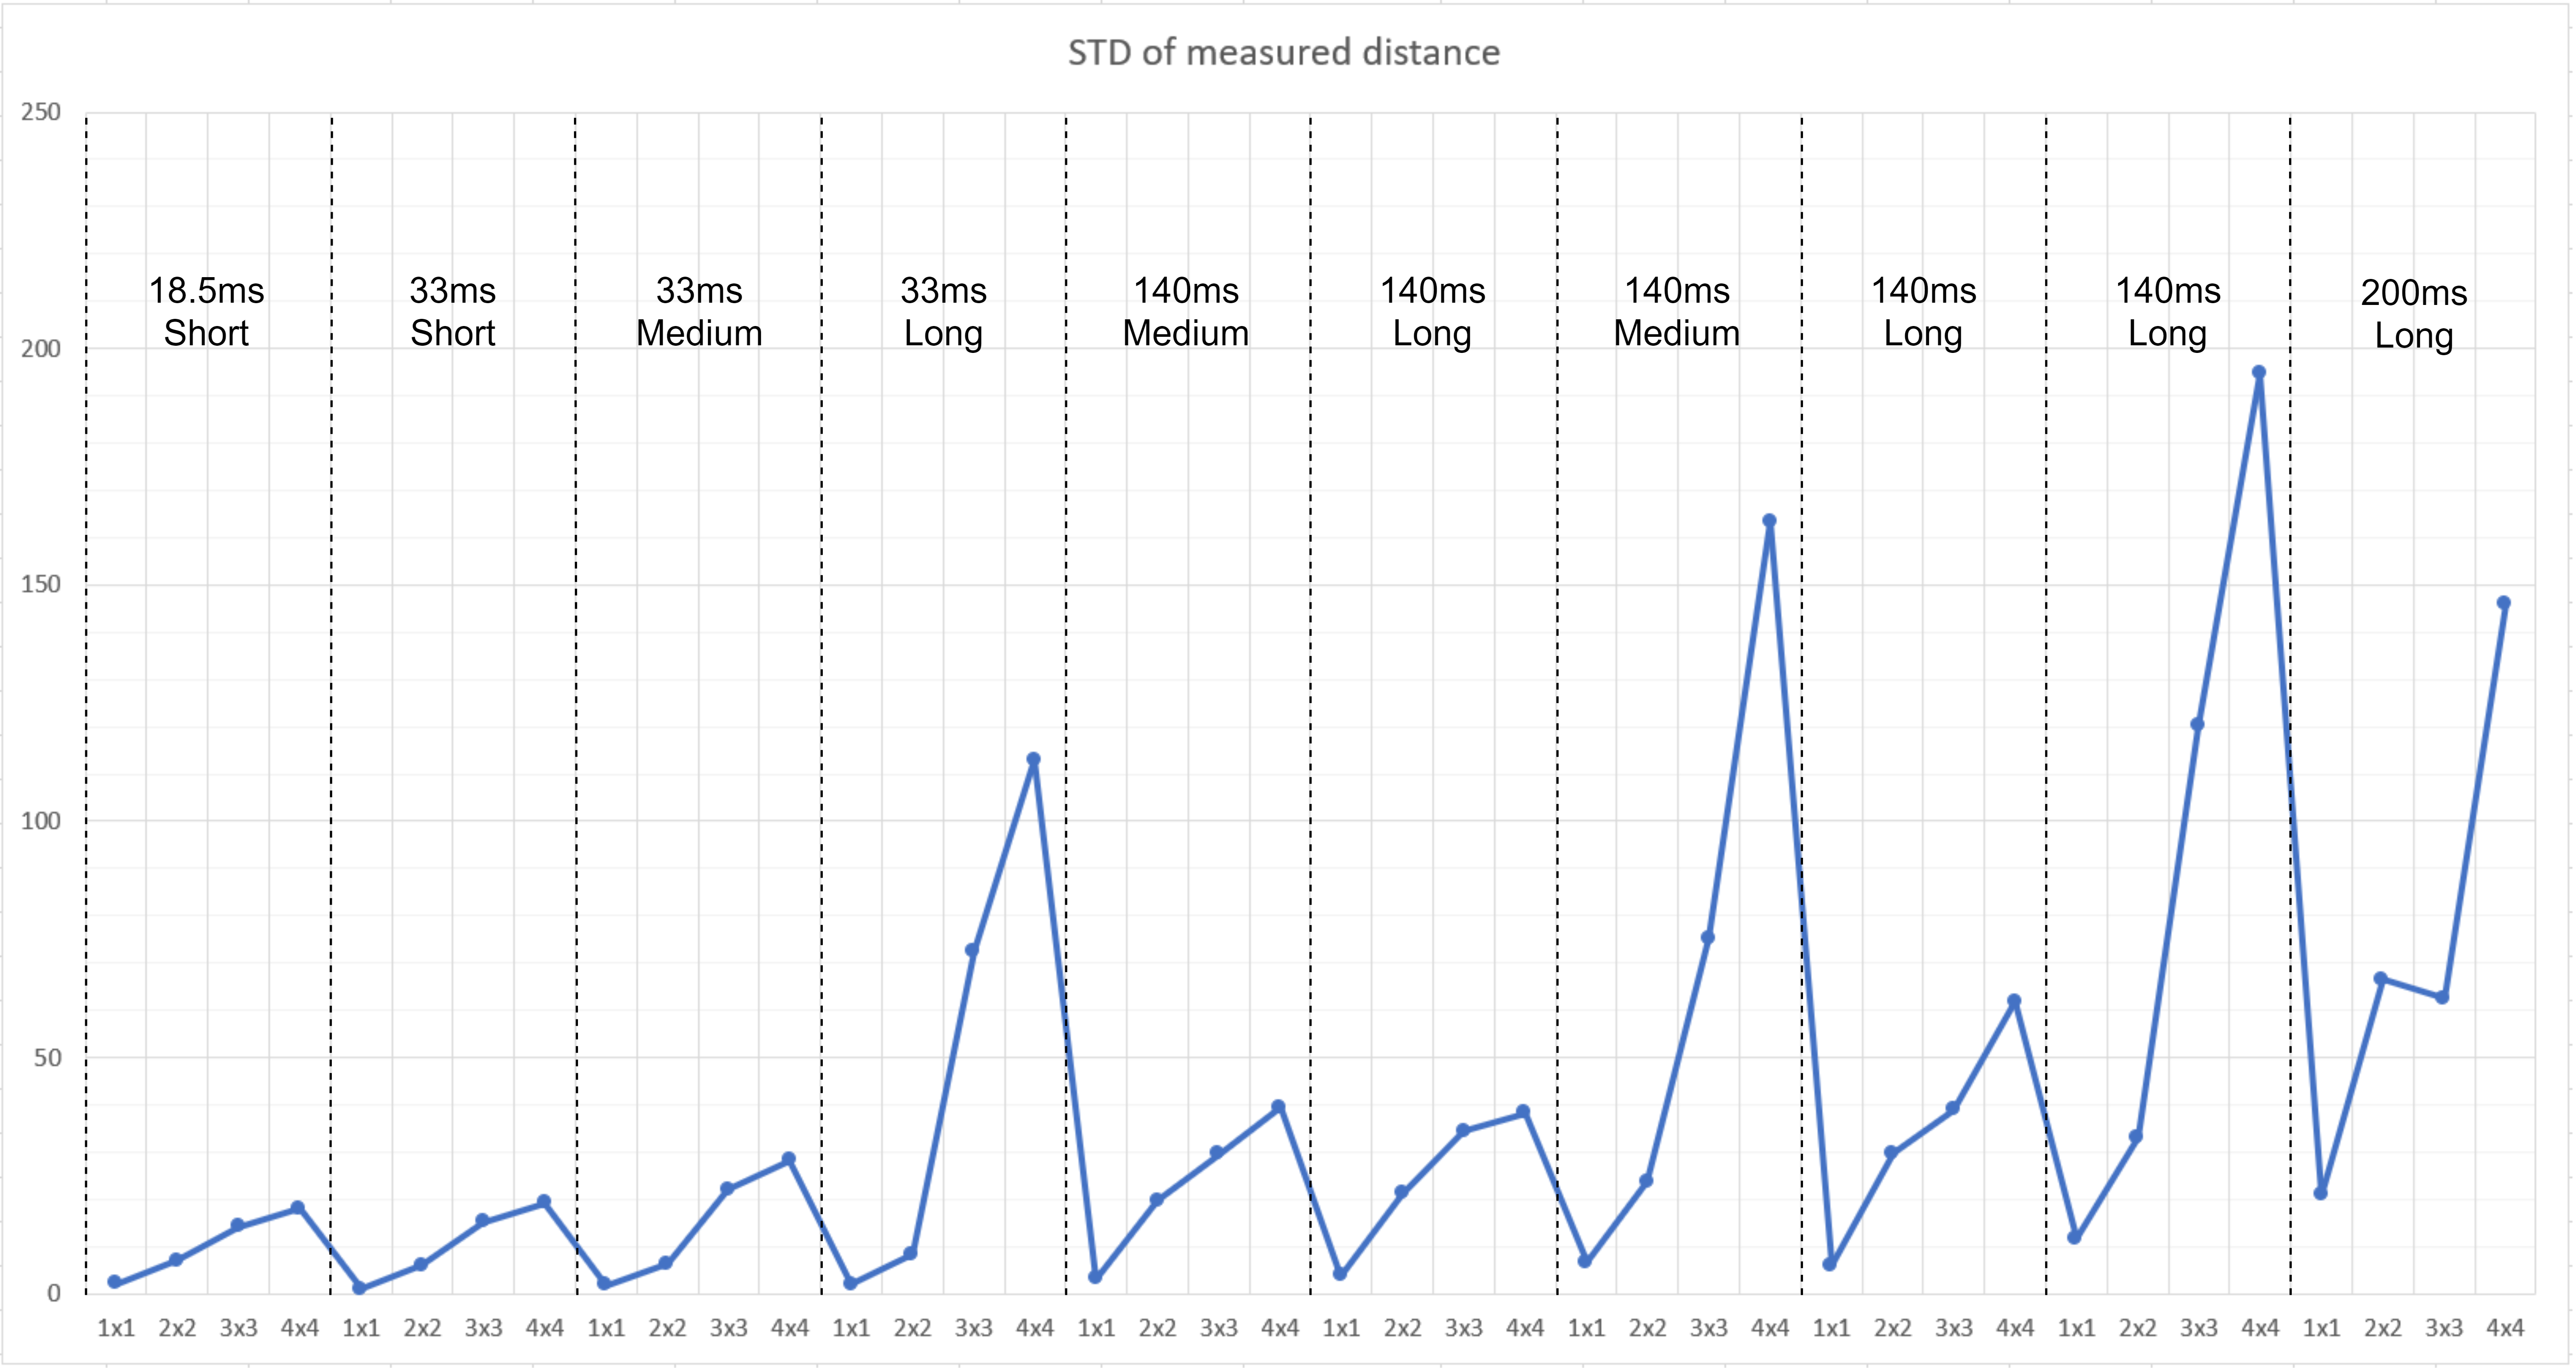
\includegraphics[width=150mm, keepaspectratio]{figures/vl53l1x_measurements_opmodes_std.png}
    \caption{VL53L1X range standard deviation in different operation modes}
    \label{fig:vl53l1x_meas_opmodes_std}
\end{figure}

\subsection{Detailed distance measurements}
Based on the measurements described in the previous section, I chose a small set of LIDAR settings 
to further investigate and see how these behave on different distances. These settings are 
candidates to be used in simulations. The goal with the setting selection is to chose the ones
that may have greater affect the SLAM performance.

After the initial tests with Cartographer SLAM, it's safe to assume that sampling time shouldn't be
greater than 500ms. This is not a strict threshold, but with a higher sampling time, the algorithm 
would have a hard time to follow the position of the drone and insert new scans precisely. The second
assumption is that more points per scan increase the performance of scan insertion, because more points
create a more detailed and therefore more unique image. 

I chose 5 setups for further investigation, 4 with each resolution and the fastest one with 18.5ms 
timing budget. The lowest timing budget to be used with 4x4 resolution is 33ms, that is expected to be
just under the previously described threshold of 500ms per scan. The same budget is chosen for 3x3 
resolution, while 2x2 has lower number of ranges per scan so a higher budget, 70ms is selected to 
have more accurate measurements. As for 1x1 18.5ms and 140ms timing budgets are selected to see
the difference between a faster and a slower setup.

Each setup has been has been measured on distances starting from 0.5m to 4m with a step size
of 0.5m. The measurements can be seen on figures \ref{fig:vl53l1x_meas_detailed_dist},
\ref{fig:vl53l1x_meas_detailed_std}, \ref{fig:vl53l1x_meas_detailed_ts}. In the end
all setups turned out to have a lower sampling time than 500ms. It is interesting, that
sampling time turned out to be higher on smaller distances and lower on high distances.
This might be because the internal algorithm of VL53L1X sensor does longer measurements
to reassure that these ranges are not artifacts coming from reflections or crosstalk.

As expected the setup with 1x1 resolution and 140ms timing budget can range the farthest 
with only 9mm standard deviation. The setup with 2x2 resolution deviates from the real 
distance by 16cm on 3.5m, but is still accurate on 3m. 
The setups with 3x3 and 4x4 resolutions can measure up to 2.5m, but deviate on farther 
measurements. 

\begin{figure}[!h]
    \centering
	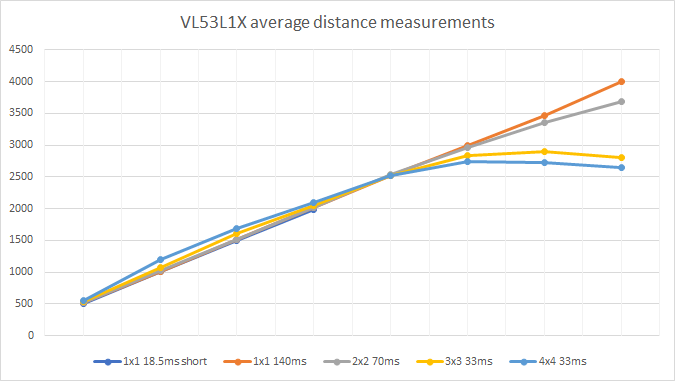
\includegraphics[width=115mm, keepaspectratio]{figures/vl53l1x_measurements_02_dist.png}
    \caption{Detailed distance measurements [mm]}
    \label{fig:vl53l1x_meas_detailed_dist}
\end{figure}

\begin{figure}[!h]
    \centering
	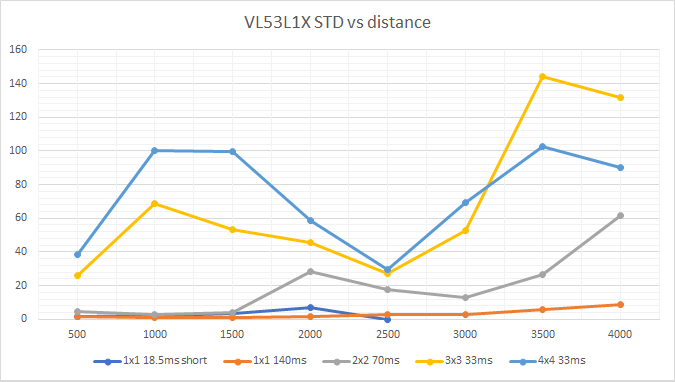
\includegraphics[width=115mm, keepaspectratio]{figures/vl53l1x_measurements_02_std.png}
    \caption{Standard deviation of selected measurements [mm]}
    \label{fig:vl53l1x_meas_detailed_std}
\end{figure}

\newpage

\begin{figure}[!h]
    \centering
	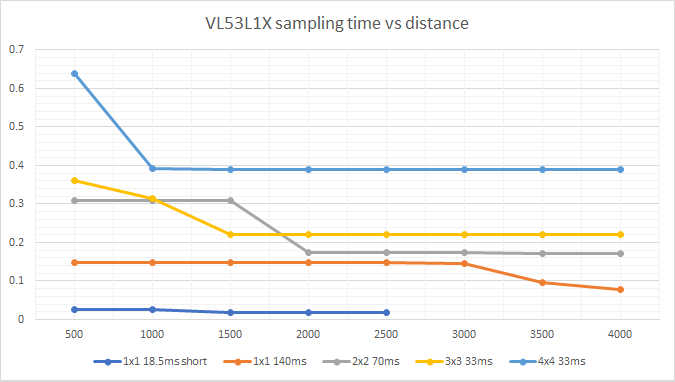
\includegraphics[width=115mm, keepaspectratio]{figures/vl53l1x_measurements_02_ts.png}
    \caption{Sampling time of selected measurements [s]}
    \label{fig:vl53l1x_meas_detailed_ts}
\end{figure}



\subsection{Detailed measurements with the fastest setup}
18.5ms timing budget with short distance preset can produce the fastest ranging measurements 
up to 1.6m according to the datasheet. The short preset also has the best ambient light 
immunity, a favorable quality. Due to these attributes I have decided to do more measurements
using these settings in combination with all resolutions.

Surprisingly the sensor with these settings was able to measure up to 2m with only 7mm 
standard deviation. Above 2m no ranges were successful, the sensor always reported 0 distance 
instead.

In comparison to the previous results the sampling time for each resolution has decreased 
significantly. In case of 4x4 resolution, the sampling time has decreased from 390ms to
265ms and the maximum distance from 2.5m to about 1m. The increase in update rate might be 
beneficial for the SLAM algorithm.

Surprisingly the update rate for 1x1 resolution reached 56Hz, that is higher than the 
maximum update rate according to the datasheet. The reason for the increased update rate
is that 50Hz was calculated using continuous measurement mode that places a 1.5ms delay
between ranges. In this scenario the device was used in single-shot mode and there was 
no delay between measurements. Although this method puts a high load on the host 
microcontroller that is not favorable in most applications.



\begin{figure}[!h]
    \centering
	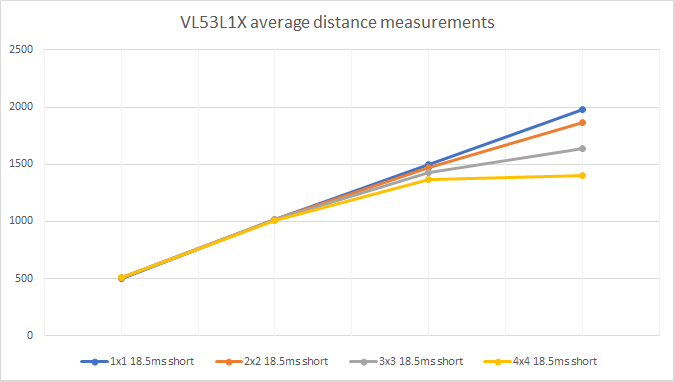
\includegraphics[width=115mm, keepaspectratio]{figures/vl53l1x_measurements_03_dist.png}
    \caption{Detailed distance measurements [mm]}
    \label{fig:vl53l1x_meas_detailed_dist}
\end{figure}

\begin{figure}[!h]
    \centering
	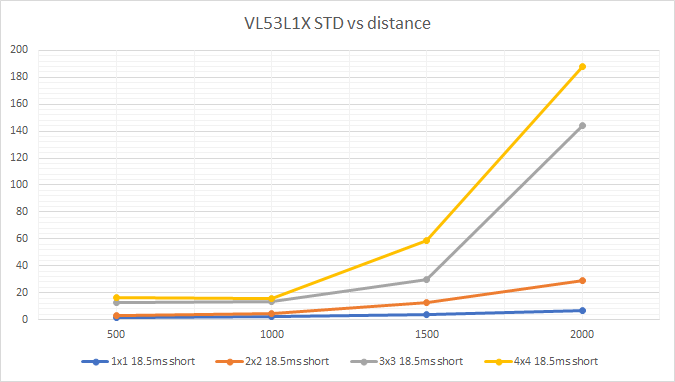
\includegraphics[width=115mm, keepaspectratio]{figures/vl53l1x_measurements_03_std.png}
    \caption{Standard deviation of selected measurements [mm]}
    \label{fig:vl53l1x_meas_detailed_std}
\end{figure}


\begin{figure}[!h]
    \centering
	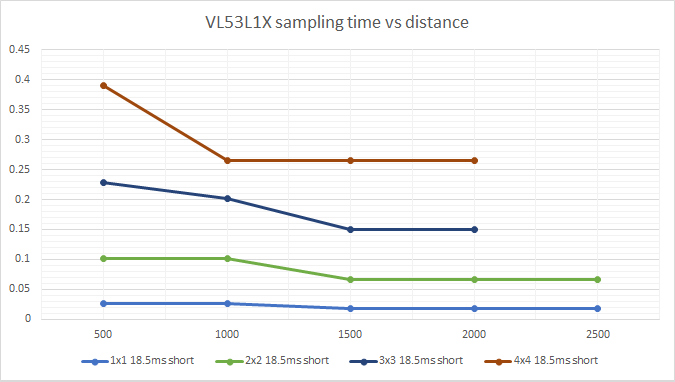
\includegraphics[width=115mm, keepaspectratio]{figures/vl53l1x_measurements_03_ts.png}
    \caption{Sampling time of selected measurements [s]}
    \label{fig:vl53l1x_meas_detailed_ts}
\end{figure}

\newpage

\section{2D SLAM evaluation}
TODO
\subsection{Unfiltered data}
TODO
\subsection{2D SLAM with 1x1 resolution}
TODO
\subsection{2D SLAM with 4x4 resolution}
TODO

\section{3D SLAM evaluation}
TODO
\subsection{Unfiltered data}
TODO
\subsection{1x1 resolution}
TODO
\subsection{4x4 resolution}
TODO